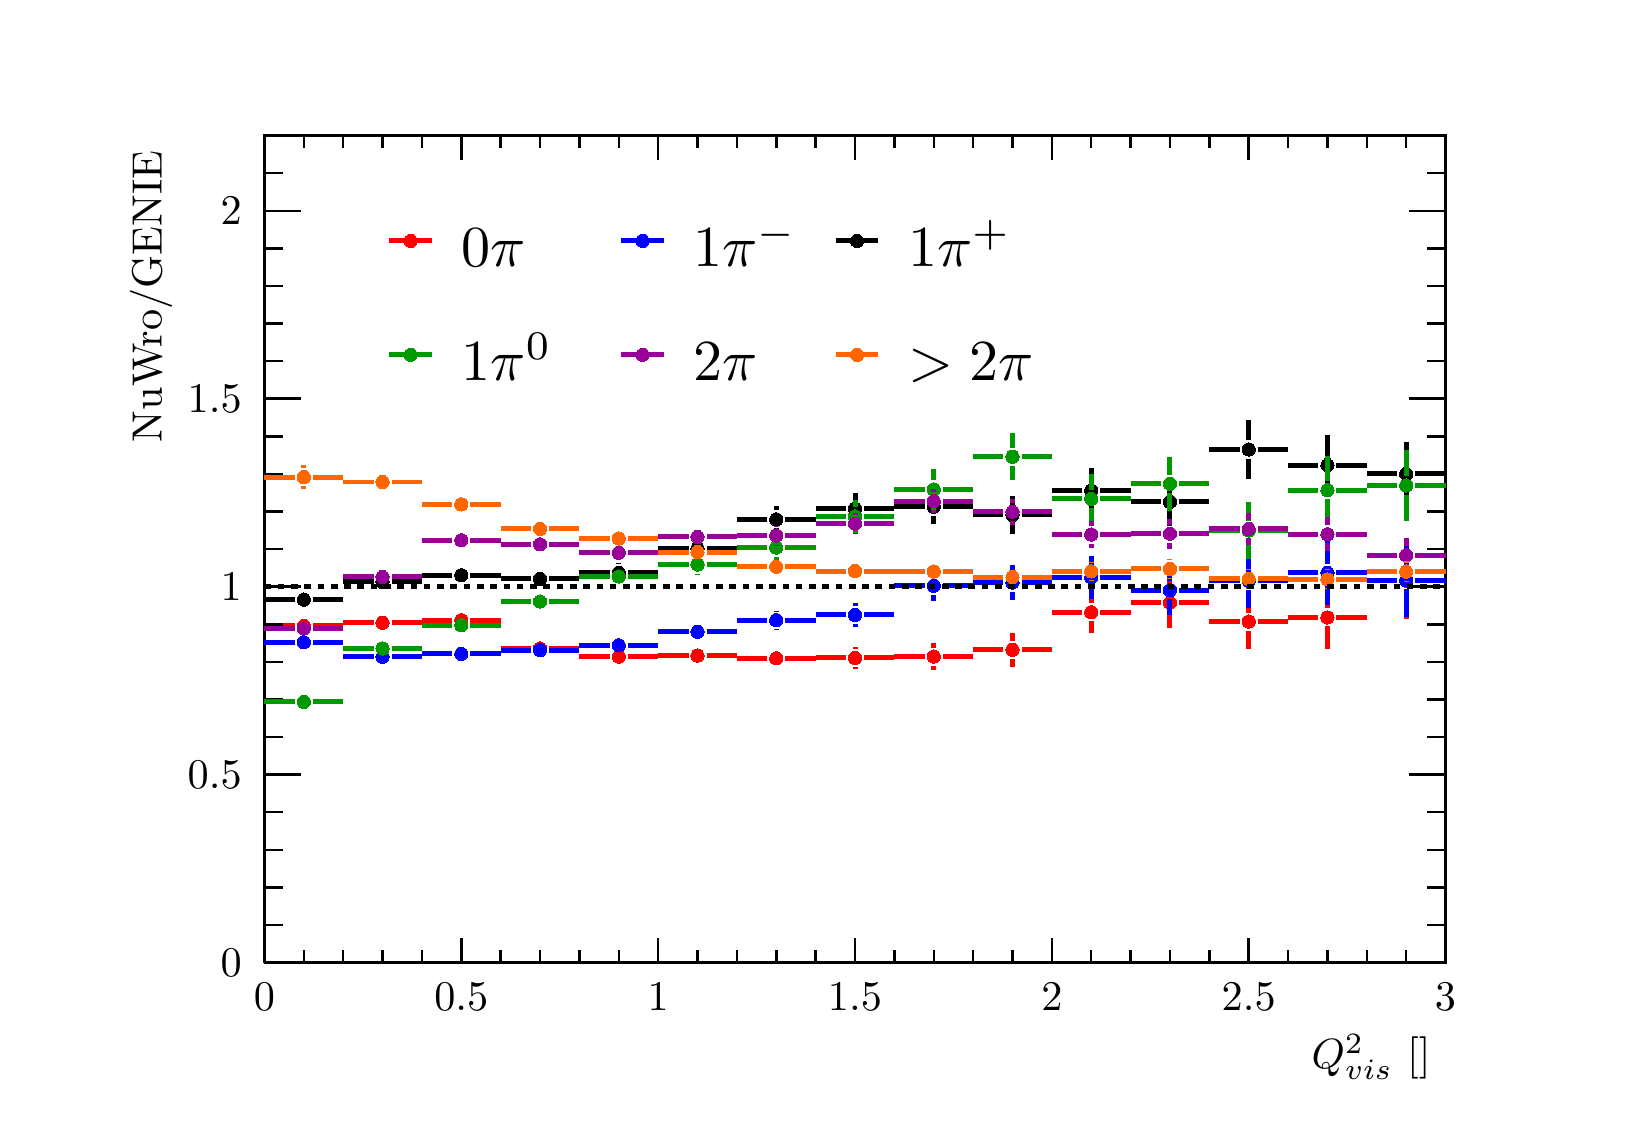
\begin{tikzpicture}
\pgfdeclareplotmark{cross} {
\pgfpathmoveto{\pgfpoint{-0.3\pgfplotmarksize}{\pgfplotmarksize}}
\pgfpathlineto{\pgfpoint{+0.3\pgfplotmarksize}{\pgfplotmarksize}}
\pgfpathlineto{\pgfpoint{+0.3\pgfplotmarksize}{0.3\pgfplotmarksize}}
\pgfpathlineto{\pgfpoint{+1\pgfplotmarksize}{0.3\pgfplotmarksize}}
\pgfpathlineto{\pgfpoint{+1\pgfplotmarksize}{-0.3\pgfplotmarksize}}
\pgfpathlineto{\pgfpoint{+0.3\pgfplotmarksize}{-0.3\pgfplotmarksize}}
\pgfpathlineto{\pgfpoint{+0.3\pgfplotmarksize}{-1.\pgfplotmarksize}}
\pgfpathlineto{\pgfpoint{-0.3\pgfplotmarksize}{-1.\pgfplotmarksize}}
\pgfpathlineto{\pgfpoint{-0.3\pgfplotmarksize}{-0.3\pgfplotmarksize}}
\pgfpathlineto{\pgfpoint{-1.\pgfplotmarksize}{-0.3\pgfplotmarksize}}
\pgfpathlineto{\pgfpoint{-1.\pgfplotmarksize}{0.3\pgfplotmarksize}}
\pgfpathlineto{\pgfpoint{-0.3\pgfplotmarksize}{0.3\pgfplotmarksize}}
\pgfpathclose
\pgfusepathqstroke
}
\pgfdeclareplotmark{cross*} {
\pgfpathmoveto{\pgfpoint{-0.3\pgfplotmarksize}{\pgfplotmarksize}}
\pgfpathlineto{\pgfpoint{+0.3\pgfplotmarksize}{\pgfplotmarksize}}
\pgfpathlineto{\pgfpoint{+0.3\pgfplotmarksize}{0.3\pgfplotmarksize}}
\pgfpathlineto{\pgfpoint{+1\pgfplotmarksize}{0.3\pgfplotmarksize}}
\pgfpathlineto{\pgfpoint{+1\pgfplotmarksize}{-0.3\pgfplotmarksize}}
\pgfpathlineto{\pgfpoint{+0.3\pgfplotmarksize}{-0.3\pgfplotmarksize}}
\pgfpathlineto{\pgfpoint{+0.3\pgfplotmarksize}{-1.\pgfplotmarksize}}
\pgfpathlineto{\pgfpoint{-0.3\pgfplotmarksize}{-1.\pgfplotmarksize}}
\pgfpathlineto{\pgfpoint{-0.3\pgfplotmarksize}{-0.3\pgfplotmarksize}}
\pgfpathlineto{\pgfpoint{-1.\pgfplotmarksize}{-0.3\pgfplotmarksize}}
\pgfpathlineto{\pgfpoint{-1.\pgfplotmarksize}{0.3\pgfplotmarksize}}
\pgfpathlineto{\pgfpoint{-0.3\pgfplotmarksize}{0.3\pgfplotmarksize}}
\pgfpathclose
\pgfusepathqfillstroke
}
\pgfdeclareplotmark{newstar} {
\pgfpathmoveto{\pgfqpoint{0pt}{\pgfplotmarksize}}
\pgfpathlineto{\pgfqpointpolar{44}{0.5\pgfplotmarksize}}
\pgfpathlineto{\pgfqpointpolar{18}{\pgfplotmarksize}}
\pgfpathlineto{\pgfqpointpolar{-20}{0.5\pgfplotmarksize}}
\pgfpathlineto{\pgfqpointpolar{-54}{\pgfplotmarksize}}
\pgfpathlineto{\pgfqpointpolar{-90}{0.5\pgfplotmarksize}}
\pgfpathlineto{\pgfqpointpolar{234}{\pgfplotmarksize}}
\pgfpathlineto{\pgfqpointpolar{198}{0.5\pgfplotmarksize}}
\pgfpathlineto{\pgfqpointpolar{162}{\pgfplotmarksize}}
\pgfpathlineto{\pgfqpointpolar{134}{0.5\pgfplotmarksize}}
\pgfpathclose
\pgfusepathqstroke
}
\pgfdeclareplotmark{newstar*} {
\pgfpathmoveto{\pgfqpoint{0pt}{\pgfplotmarksize}}
\pgfpathlineto{\pgfqpointpolar{44}{0.5\pgfplotmarksize}}
\pgfpathlineto{\pgfqpointpolar{18}{\pgfplotmarksize}}
\pgfpathlineto{\pgfqpointpolar{-20}{0.5\pgfplotmarksize}}
\pgfpathlineto{\pgfqpointpolar{-54}{\pgfplotmarksize}}
\pgfpathlineto{\pgfqpointpolar{-90}{0.5\pgfplotmarksize}}
\pgfpathlineto{\pgfqpointpolar{234}{\pgfplotmarksize}}
\pgfpathlineto{\pgfqpointpolar{198}{0.5\pgfplotmarksize}}
\pgfpathlineto{\pgfqpointpolar{162}{\pgfplotmarksize}}
\pgfpathlineto{\pgfqpointpolar{134}{0.5\pgfplotmarksize}}
\pgfpathclose
\pgfusepathqfillstroke
}
\definecolor{c}{rgb}{1,1,1};
\draw [color=c, fill=c] (0,0) rectangle (20,13.639);
\draw [color=c, fill=c] (3,1.77307) rectangle (18,12.2751);
\definecolor{c}{rgb}{0,0,0};
\draw [c,line width=0.9] (3,1.77307) -- (3,12.2751) -- (18,12.2751) -- (18,1.77307) -- (3,1.77307);
\definecolor{c}{rgb}{1,1,1};
\draw [color=c, fill=c] (3,1.77307) rectangle (18,12.2751);
\definecolor{c}{rgb}{0,0,0};
\draw [c,line width=0.9] (3,1.77307) -- (3,12.2751) -- (18,12.2751) -- (18,1.77307) -- (3,1.77307);
\definecolor{c}{rgb}{1,0,0};
\draw [c,line width=1.8] (3,6.04743) -- (3.38539,6.04743);
\draw [c,line width=1.8] (3.61461,6.04743) -- (4,6.04743);
\foreach \P in {(3.5,6.04743)}{\draw[mark options={color=c,fill=c},mark size=2.402402pt, line width=0.000000pt, mark=*] plot coordinates {\P};}
\draw [c,line width=1.8] (4,6.08852) -- (4.38539,6.08852);
\draw [c,line width=1.8] (4.61461,6.08852) -- (5,6.08852);
\foreach \P in {(4.5,6.08852)}{\draw[mark options={color=c,fill=c},mark size=2.402402pt, line width=0.000000pt, mark=*] plot coordinates {\P};}
\draw [c,line width=1.8] (5,6.12089) -- (5.38539,6.12089);
\draw [c,line width=1.8] (5.61461,6.12089) -- (6,6.12089);
\foreach \P in {(5.5,6.12089)}{\draw[mark options={color=c,fill=c},mark size=2.402402pt, line width=0.000000pt, mark=*] plot coordinates {\P};}
\draw [c,line width=1.8] (6,5.76282) -- (6.38539,5.76282);
\draw [c,line width=1.8] (6.61461,5.76282) -- (7,5.76282);
\foreach \P in {(6.5,5.76282)}{\draw[mark options={color=c,fill=c},mark size=2.402402pt, line width=0.000000pt, mark=*] plot coordinates {\P};}
\draw [c,line width=1.8] (7,5.65759) -- (7.38539,5.65759);
\draw [c,line width=1.8] (7.61461,5.65759) -- (8,5.65759);
\foreach \P in {(7.5,5.65759)}{\draw[mark options={color=c,fill=c},mark size=2.402402pt, line width=0.000000pt, mark=*] plot coordinates {\P};}
\draw [c,line width=1.8] (8,5.6708) -- (8.38539,5.6708);
\draw [c,line width=1.8] (8.61461,5.6708) -- (9,5.6708);
\foreach \P in {(8.5,5.6708)}{\draw[mark options={color=c,fill=c},mark size=2.402402pt, line width=0.000000pt, mark=*] plot coordinates {\P};}
\draw [c,line width=1.8] (9,5.63729) -- (9.38539,5.63729);
\draw [c,line width=1.8] (9.61461,5.63729) -- (10,5.63729);
\foreach \P in {(9.5,5.63729)}{\draw[mark options={color=c,fill=c},mark size=2.402402pt, line width=0.000000pt, mark=*] plot coordinates {\P};}
\draw [c,line width=1.8] (10.5,5.50269) -- (10.5,5.52734);
\draw [c,line width=1.8] (10.5,5.75657) -- (10.5,5.78122);
\draw [c,line width=1.8] (10,5.64196) -- (10.3854,5.64196);
\draw [c,line width=1.8] (10.6146,5.64196) -- (11,5.64196);
\foreach \P in {(10.5,5.64196)}{\draw[mark options={color=c,fill=c},mark size=2.402402pt, line width=0.000000pt, mark=*] plot coordinates {\P};}
\draw [c,line width=1.8] (11.5,5.48713) -- (11.5,5.54456);
\draw [c,line width=1.8] (11.5,5.77379) -- (11.5,5.83122);
\draw [c,line width=1.8] (11,5.65918) -- (11.3854,5.65918);
\draw [c,line width=1.8] (11.6146,5.65918) -- (12,5.65918);
\foreach \P in {(11.5,5.65918)}{\draw[mark options={color=c,fill=c},mark size=2.402402pt, line width=0.000000pt, mark=*] plot coordinates {\P};}
\draw [c,line width=1.8] (12.5,5.53191) -- (12.5,5.63008);
\draw [c,line width=1.8] (12.5,5.8593) -- (12.5,5.95747);
\draw [c,line width=1.8] (12,5.74469) -- (12.3854,5.74469);
\draw [c,line width=1.8] (12.6146,5.74469) -- (13,5.74469);
\foreach \P in {(12.5,5.74469)}{\draw[mark options={color=c,fill=c},mark size=2.402402pt, line width=0.000000pt, mark=*] plot coordinates {\P};}
\draw [c,line width=1.8] (13.5,5.95411) -- (13.5,6.10723);
\draw [c,line width=1.8] (13.5,6.33645) -- (13.5,6.48956);
\draw [c,line width=1.8] (13,6.22184) -- (13.3854,6.22184);
\draw [c,line width=1.8] (13.6146,6.22184) -- (14,6.22184);
\foreach \P in {(13.5,6.22184)}{\draw[mark options={color=c,fill=c},mark size=2.402402pt, line width=0.000000pt, mark=*] plot coordinates {\P};}
\draw [c,line width=1.8] (14.5,6.02788) -- (14.5,6.22779);
\draw [c,line width=1.8] (14.5,6.45701) -- (14.5,6.65692);
\draw [c,line width=1.8] (14,6.3424) -- (14.3854,6.3424);
\draw [c,line width=1.8] (14.6146,6.3424) -- (15,6.3424);
\foreach \P in {(14.5,6.3424)}{\draw[mark options={color=c,fill=c},mark size=2.402402pt, line width=0.000000pt, mark=*] plot coordinates {\P};}
\draw [c,line width=1.8] (15.5,5.75695) -- (15.5,5.98918);
\draw [c,line width=1.8] (15.5,6.21841) -- (15.5,6.45065);
\draw [c,line width=1.8] (15,6.1038) -- (15.3854,6.1038);
\draw [c,line width=1.8] (15.6146,6.1038) -- (16,6.1038);
\foreach \P in {(15.5,6.1038)}{\draw[mark options={color=c,fill=c},mark size=2.402402pt, line width=0.000000pt, mark=*] plot coordinates {\P};}
\draw [c,line width=1.8] (16.5,5.76141) -- (16.5,6.04106);
\draw [c,line width=1.8] (16.5,6.27029) -- (16.5,6.54995);
\draw [c,line width=1.8] (16,6.15568) -- (16.3854,6.15568);
\draw [c,line width=1.8] (16.6146,6.15568) -- (17,6.15568);
\foreach \P in {(16.5,6.15568)}{\draw[mark options={color=c,fill=c},mark size=2.402402pt, line width=0.000000pt, mark=*] plot coordinates {\P};}
\draw [c,line width=1.8] (17.5,6.13333) -- (17.5,6.50904);
\draw [c,line width=1.8] (17.5,6.73827) -- (17.5,7.11399);
\draw [c,line width=1.8] (17,6.62366) -- (17.3854,6.62366);
\draw [c,line width=1.8] (17.6146,6.62366) -- (18,6.62366);
\foreach \P in {(17.5,6.62366)}{\draw[mark options={color=c,fill=c},mark size=2.402402pt, line width=0.000000pt, mark=*] plot coordinates {\P};}
\definecolor{c}{rgb}{0,0,0};
\draw [c,line width=0.9] (3,1.77307) -- (18,1.77307);
\draw [c,line width=0.9] (3,2.07994) -- (3,1.77307);
\draw [c,line width=0.9] (3.5,1.9265) -- (3.5,1.77307);
\draw [c,line width=0.9] (4,1.9265) -- (4,1.77307);
\draw [c,line width=0.9] (4.5,1.9265) -- (4.5,1.77307);
\draw [c,line width=0.9] (5,1.9265) -- (5,1.77307);
\draw [c,line width=0.9] (5.5,2.07994) -- (5.5,1.77307);
\draw [c,line width=0.9] (6,1.9265) -- (6,1.77307);
\draw [c,line width=0.9] (6.5,1.9265) -- (6.5,1.77307);
\draw [c,line width=0.9] (7,1.9265) -- (7,1.77307);
\draw [c,line width=0.9] (7.5,1.9265) -- (7.5,1.77307);
\draw [c,line width=0.9] (8,2.07994) -- (8,1.77307);
\draw [c,line width=0.9] (8.5,1.9265) -- (8.5,1.77307);
\draw [c,line width=0.9] (9,1.9265) -- (9,1.77307);
\draw [c,line width=0.9] (9.5,1.9265) -- (9.5,1.77307);
\draw [c,line width=0.9] (10,1.9265) -- (10,1.77307);
\draw [c,line width=0.9] (10.5,2.07994) -- (10.5,1.77307);
\draw [c,line width=0.9] (11,1.9265) -- (11,1.77307);
\draw [c,line width=0.9] (11.5,1.9265) -- (11.5,1.77307);
\draw [c,line width=0.9] (12,1.9265) -- (12,1.77307);
\draw [c,line width=0.9] (12.5,1.9265) -- (12.5,1.77307);
\draw [c,line width=0.9] (13,2.07994) -- (13,1.77307);
\draw [c,line width=0.9] (13.5,1.9265) -- (13.5,1.77307);
\draw [c,line width=0.9] (14,1.9265) -- (14,1.77307);
\draw [c,line width=0.9] (14.5,1.9265) -- (14.5,1.77307);
\draw [c,line width=0.9] (15,1.9265) -- (15,1.77307);
\draw [c,line width=0.9] (15.5,2.07994) -- (15.5,1.77307);
\draw [c,line width=0.9] (16,1.9265) -- (16,1.77307);
\draw [c,line width=0.9] (16.5,1.9265) -- (16.5,1.77307);
\draw [c,line width=0.9] (17,1.9265) -- (17,1.77307);
\draw [c,line width=0.9] (17.5,1.9265) -- (17.5,1.77307);
\draw [c,line width=0.9] (18,2.07994) -- (18,1.77307);
\draw [c,line width=0.9] (18,2.07994) -- (18,1.77307);
\draw [anchor=base] (3,1.15931) node[scale=1.52731, color=c, rotate=0]{0};
\draw [anchor=base] (5.5,1.15931) node[scale=1.52731, color=c, rotate=0]{0.5};
\draw [anchor=base] (8,1.15931) node[scale=1.52731, color=c, rotate=0]{1};
\draw [anchor=base] (10.5,1.15931) node[scale=1.52731, color=c, rotate=0]{1.5};
\draw [anchor=base] (13,1.15931) node[scale=1.52731, color=c, rotate=0]{2};
\draw [anchor=base] (15.5,1.15931) node[scale=1.52731, color=c, rotate=0]{2.5};
\draw [anchor=base] (18,1.15931) node[scale=1.52731, color=c, rotate=0]{3};
\draw [anchor= east] (18,0.572837) node[scale=1.52731, color=c, rotate=0]{ $Q^{2}_{\text{vis}}$ [\si{\giga\electronvolt\squared}] };
\draw [c,line width=0.9] (3,12.2751) -- (18,12.2751);
\draw [c,line width=0.9] (3,11.9682) -- (3,12.2751);
\draw [c,line width=0.9] (3.5,12.1216) -- (3.5,12.2751);
\draw [c,line width=0.9] (4,12.1216) -- (4,12.2751);
\draw [c,line width=0.9] (4.5,12.1216) -- (4.5,12.2751);
\draw [c,line width=0.9] (5,12.1216) -- (5,12.2751);
\draw [c,line width=0.9] (5.5,11.9682) -- (5.5,12.2751);
\draw [c,line width=0.9] (6,12.1216) -- (6,12.2751);
\draw [c,line width=0.9] (6.5,12.1216) -- (6.5,12.2751);
\draw [c,line width=0.9] (7,12.1216) -- (7,12.2751);
\draw [c,line width=0.9] (7.5,12.1216) -- (7.5,12.2751);
\draw [c,line width=0.9] (8,11.9682) -- (8,12.2751);
\draw [c,line width=0.9] (8.5,12.1216) -- (8.5,12.2751);
\draw [c,line width=0.9] (9,12.1216) -- (9,12.2751);
\draw [c,line width=0.9] (9.5,12.1216) -- (9.5,12.2751);
\draw [c,line width=0.9] (10,12.1216) -- (10,12.2751);
\draw [c,line width=0.9] (10.5,11.9682) -- (10.5,12.2751);
\draw [c,line width=0.9] (11,12.1216) -- (11,12.2751);
\draw [c,line width=0.9] (11.5,12.1216) -- (11.5,12.2751);
\draw [c,line width=0.9] (12,12.1216) -- (12,12.2751);
\draw [c,line width=0.9] (12.5,12.1216) -- (12.5,12.2751);
\draw [c,line width=0.9] (13,11.9682) -- (13,12.2751);
\draw [c,line width=0.9] (13.5,12.1216) -- (13.5,12.2751);
\draw [c,line width=0.9] (14,12.1216) -- (14,12.2751);
\draw [c,line width=0.9] (14.5,12.1216) -- (14.5,12.2751);
\draw [c,line width=0.9] (15,12.1216) -- (15,12.2751);
\draw [c,line width=0.9] (15.5,11.9682) -- (15.5,12.2751);
\draw [c,line width=0.9] (16,12.1216) -- (16,12.2751);
\draw [c,line width=0.9] (16.5,12.1216) -- (16.5,12.2751);
\draw [c,line width=0.9] (17,12.1216) -- (17,12.2751);
\draw [c,line width=0.9] (17.5,12.1216) -- (17.5,12.2751);
\draw [c,line width=0.9] (18,11.9682) -- (18,12.2751);
\draw [c,line width=0.9] (18,11.9682) -- (18,12.2751);
\draw [c,line width=0.9] (3,1.77307) -- (3,12.2751);
\draw [c,line width=0.9] (3.462,1.77307) -- (3,1.77307);
\draw [c,line width=0.9] (3.231,2.25043) -- (3,2.25043);
\draw [c,line width=0.9] (3.231,2.72779) -- (3,2.72779);
\draw [c,line width=0.9] (3.231,3.20516) -- (3,3.20516);
\draw [c,line width=0.9] (3.231,3.68252) -- (3,3.68252);
\draw [c,line width=0.9] (3.462,4.15989) -- (3,4.15989);
\draw [c,line width=0.9] (3.231,4.63725) -- (3,4.63725);
\draw [c,line width=0.9] (3.231,5.11461) -- (3,5.11461);
\draw [c,line width=0.9] (3.231,5.59198) -- (3,5.59198);
\draw [c,line width=0.9] (3.231,6.06934) -- (3,6.06934);
\draw [c,line width=0.9] (3.462,6.5467) -- (3,6.5467);
\draw [c,line width=0.9] (3.231,7.02407) -- (3,7.02407);
\draw [c,line width=0.9] (3.231,7.50143) -- (3,7.50143);
\draw [c,line width=0.9] (3.231,7.9788) -- (3,7.9788);
\draw [c,line width=0.9] (3.231,8.45616) -- (3,8.45616);
\draw [c,line width=0.9] (3.462,8.93352) -- (3,8.93352);
\draw [c,line width=0.9] (3.231,9.41089) -- (3,9.41089);
\draw [c,line width=0.9] (3.231,9.88825) -- (3,9.88825);
\draw [c,line width=0.9] (3.231,10.3656) -- (3,10.3656);
\draw [c,line width=0.9] (3.231,10.843) -- (3,10.843);
\draw [c,line width=0.9] (3.462,11.3203) -- (3,11.3203);
\draw [c,line width=0.9] (3.462,11.3203) -- (3,11.3203);
\draw [c,line width=0.9] (3.231,11.7977) -- (3,11.7977);
\draw [c,line width=0.9] (3.231,12.2751) -- (3,12.2751);
\draw [anchor= east] (2.9,1.77307) node[scale=1.52731, color=c, rotate=0]{0};
\draw [anchor= east] (2.9,4.15989) node[scale=1.52731, color=c, rotate=0]{0.5};
\draw [anchor= east] (2.9,6.5467) node[scale=1.52731, color=c, rotate=0]{1};
\draw [anchor= east] (2.9,8.93352) node[scale=1.52731, color=c, rotate=0]{1.5};
\draw [anchor= east] (2.9,11.3203) node[scale=1.52731, color=c, rotate=0]{2};
\draw [anchor= east] (1.56,12.2751) node[scale=1.52731, color=c, rotate=90]{ NuWro/GENIE};
\draw [c,line width=0.9] (18,1.77307) -- (18,12.2751);
\draw [c,line width=0.9] (17.538,1.77307) -- (18,1.77307);
\draw [c,line width=0.9] (17.769,2.25043) -- (18,2.25043);
\draw [c,line width=0.9] (17.769,2.72779) -- (18,2.72779);
\draw [c,line width=0.9] (17.769,3.20516) -- (18,3.20516);
\draw [c,line width=0.9] (17.769,3.68252) -- (18,3.68252);
\draw [c,line width=0.9] (17.538,4.15989) -- (18,4.15989);
\draw [c,line width=0.9] (17.769,4.63725) -- (18,4.63725);
\draw [c,line width=0.9] (17.769,5.11461) -- (18,5.11461);
\draw [c,line width=0.9] (17.769,5.59198) -- (18,5.59198);
\draw [c,line width=0.9] (17.769,6.06934) -- (18,6.06934);
\draw [c,line width=0.9] (17.538,6.5467) -- (18,6.5467);
\draw [c,line width=0.9] (17.769,7.02407) -- (18,7.02407);
\draw [c,line width=0.9] (17.769,7.50143) -- (18,7.50143);
\draw [c,line width=0.9] (17.769,7.9788) -- (18,7.9788);
\draw [c,line width=0.9] (17.769,8.45616) -- (18,8.45616);
\draw [c,line width=0.9] (17.538,8.93352) -- (18,8.93352);
\draw [c,line width=0.9] (17.769,9.41089) -- (18,9.41089);
\draw [c,line width=0.9] (17.769,9.88825) -- (18,9.88825);
\draw [c,line width=0.9] (17.769,10.3656) -- (18,10.3656);
\draw [c,line width=0.9] (17.769,10.843) -- (18,10.843);
\draw [c,line width=0.9] (17.538,11.3203) -- (18,11.3203);
\draw [c,line width=0.9] (17.538,11.3203) -- (18,11.3203);
\draw [c,line width=0.9] (17.769,11.7977) -- (18,11.7977);
\draw [c,line width=0.9] (17.769,12.2751) -- (18,12.2751);
\definecolor{c}{rgb}{0,0,1};
\draw [c,line width=1.8] (3,5.8411) -- (3.38539,5.8411);
\draw [c,line width=1.8] (3.61461,5.8411) -- (4,5.8411);
\foreach \P in {(3.5,5.8411)}{\draw[mark options={color=c,fill=c},mark size=2.402402pt, line width=0.000000pt, mark=*] plot coordinates {\P};}
\draw [c,line width=1.8] (4,5.65657) -- (4.38539,5.65657);
\draw [c,line width=1.8] (4.61461,5.65657) -- (5,5.65657);
\foreach \P in {(4.5,5.65657)}{\draw[mark options={color=c,fill=c},mark size=2.402402pt, line width=0.000000pt, mark=*] plot coordinates {\P};}
\draw [c,line width=1.8] (5,5.69388) -- (5.38539,5.69388);
\draw [c,line width=1.8] (5.61461,5.69388) -- (6,5.69388);
\foreach \P in {(5.5,5.69388)}{\draw[mark options={color=c,fill=c},mark size=2.402402pt, line width=0.000000pt, mark=*] plot coordinates {\P};}
\draw [c,line width=1.8] (6,5.74041) -- (6.38539,5.74041);
\draw [c,line width=1.8] (6.61461,5.74041) -- (7,5.74041);
\foreach \P in {(6.5,5.74041)}{\draw[mark options={color=c,fill=c},mark size=2.402402pt, line width=0.000000pt, mark=*] plot coordinates {\P};}
\draw [c,line width=1.8] (7,5.80259) -- (7.38539,5.80259);
\draw [c,line width=1.8] (7.61461,5.80259) -- (8,5.80259);
\foreach \P in {(7.5,5.80259)}{\draw[mark options={color=c,fill=c},mark size=2.402402pt, line width=0.000000pt, mark=*] plot coordinates {\P};}
\draw [c,line width=1.8] (8,5.97399) -- (8.38539,5.97399);
\draw [c,line width=1.8] (8.61461,5.97399) -- (9,5.97399);
\foreach \P in {(8.5,5.97399)}{\draw[mark options={color=c,fill=c},mark size=2.402402pt, line width=0.000000pt, mark=*] plot coordinates {\P};}
\draw [c,line width=1.8] (9.5,5.99969) -- (9.5,6.00656);
\draw [c,line width=1.8] (9.5,6.23578) -- (9.5,6.24265);
\draw [c,line width=1.8] (9,6.12117) -- (9.38539,6.12117);
\draw [c,line width=1.8] (9.61461,6.12117) -- (10,6.12117);
\foreach \P in {(9.5,6.12117)}{\draw[mark options={color=c,fill=c},mark size=2.402402pt, line width=0.000000pt, mark=*] plot coordinates {\P};}
\draw [c,line width=1.8] (10.5,6.0396) -- (10.5,6.07429);
\draw [c,line width=1.8] (10.5,6.30352) -- (10.5,6.3382);
\draw [c,line width=1.8] (10,6.1889) -- (10.3854,6.1889);
\draw [c,line width=1.8] (10.6146,6.1889) -- (11,6.1889);
\foreach \P in {(10.5,6.1889)}{\draw[mark options={color=c,fill=c},mark size=2.402402pt, line width=0.000000pt, mark=*] plot coordinates {\P};}
\draw [c,line width=1.8] (11.5,6.36671) -- (11.5,6.44376);
\draw [c,line width=1.8] (11.5,6.67299) -- (11.5,6.75003);
\draw [c,line width=1.8] (11,6.55837) -- (11.3854,6.55837);
\draw [c,line width=1.8] (11.6146,6.55837) -- (12,6.55837);
\foreach \P in {(11.5,6.55837)}{\draw[mark options={color=c,fill=c},mark size=2.402402pt, line width=0.000000pt, mark=*] plot coordinates {\P};}
\draw [c,line width=1.8] (12.5,6.3725) -- (12.5,6.48521);
\draw [c,line width=1.8] (12.5,6.71443) -- (12.5,6.82713);
\draw [c,line width=1.8] (12,6.59982) -- (12.3854,6.59982);
\draw [c,line width=1.8] (12.6146,6.59982) -- (13,6.59982);
\foreach \P in {(12.5,6.59982)}{\draw[mark options={color=c,fill=c},mark size=2.402402pt, line width=0.000000pt, mark=*] plot coordinates {\P};}
\draw [c,line width=1.8] (13.5,6.39344) -- (13.5,6.5512);
\draw [c,line width=1.8] (13.5,6.78043) -- (13.5,6.93819);
\draw [c,line width=1.8] (13,6.66581) -- (13.3854,6.66581);
\draw [c,line width=1.8] (13.6146,6.66581) -- (14,6.66581);
\foreach \P in {(13.5,6.66581)}{\draw[mark options={color=c,fill=c},mark size=2.402402pt, line width=0.000000pt, mark=*] plot coordinates {\P};}
\draw [c,line width=1.8] (14.5,6.19266) -- (14.5,6.38715);
\draw [c,line width=1.8] (14.5,6.61638) -- (14.5,6.81087);
\draw [c,line width=1.8] (14,6.50176) -- (14.3854,6.50176);
\draw [c,line width=1.8] (14.6146,6.50176) -- (15,6.50176);
\foreach \P in {(14.5,6.50176)}{\draw[mark options={color=c,fill=c},mark size=2.402402pt, line width=0.000000pt, mark=*] plot coordinates {\P};}
\draw [c,line width=1.8] (15.5,6.27302) -- (15.5,6.50785);
\draw [c,line width=1.8] (15.5,6.73708) -- (15.5,6.9719);
\draw [c,line width=1.8] (15,6.62246) -- (15.3854,6.62246);
\draw [c,line width=1.8] (15.6146,6.62246) -- (16,6.62246);
\foreach \P in {(15.5,6.62246)}{\draw[mark options={color=c,fill=c},mark size=2.402402pt, line width=0.000000pt, mark=*] plot coordinates {\P};}
\draw [c,line width=1.8] (16.5,6.30891) -- (16.5,6.60758);
\draw [c,line width=1.8] (16.5,6.83681) -- (16.5,7.13549);
\draw [c,line width=1.8] (16,6.7222) -- (16.3854,6.7222);
\draw [c,line width=1.8] (16.6146,6.7222) -- (17,6.7222);
\foreach \P in {(16.5,6.7222)}{\draw[mark options={color=c,fill=c},mark size=2.402402pt, line width=0.000000pt, mark=*] plot coordinates {\P};}
\draw [c,line width=1.8] (17.5,6.16306) -- (17.5,6.51295);
\draw [c,line width=1.8] (17.5,6.74218) -- (17.5,7.09208);
\draw [c,line width=1.8] (17,6.62757) -- (17.3854,6.62757);
\draw [c,line width=1.8] (17.6146,6.62757) -- (18,6.62757);
\foreach \P in {(17.5,6.62757)}{\draw[mark options={color=c,fill=c},mark size=2.402402pt, line width=0.000000pt, mark=*] plot coordinates {\P};}
\definecolor{c}{rgb}{0,0,0};
\draw [c,line width=1.8] (3,6.38243) -- (3.38539,6.38243);
\draw [c,line width=1.8] (3.61461,6.38243) -- (4,6.38243);
\foreach \P in {(3.5,6.38243)}{\draw[mark options={color=c,fill=c},mark size=2.402402pt, line width=0.000000pt, mark=*] plot coordinates {\P};}
\draw [c,line width=1.8] (4,6.60756) -- (4.38539,6.60756);
\draw [c,line width=1.8] (4.61461,6.60756) -- (5,6.60756);
\foreach \P in {(4.5,6.60756)}{\draw[mark options={color=c,fill=c},mark size=2.402402pt, line width=0.000000pt, mark=*] plot coordinates {\P};}
\draw [c,line width=1.8] (5,6.69119) -- (5.38539,6.69119);
\draw [c,line width=1.8] (5.61461,6.69119) -- (6,6.69119);
\foreach \P in {(5.5,6.69119)}{\draw[mark options={color=c,fill=c},mark size=2.402402pt, line width=0.000000pt, mark=*] plot coordinates {\P};}
\draw [c,line width=1.8] (6,6.64474) -- (6.38539,6.64474);
\draw [c,line width=1.8] (6.61461,6.64474) -- (7,6.64474);
\foreach \P in {(6.5,6.64474)}{\draw[mark options={color=c,fill=c},mark size=2.402402pt, line width=0.000000pt, mark=*] plot coordinates {\P};}
\draw [c,line width=1.8] (7.5,6.60047) -- (7.5,6.60934);
\draw [c,line width=1.8] (7.5,6.83857) -- (7.5,6.84744);
\draw [c,line width=1.8] (7,6.72395) -- (7.38539,6.72395);
\draw [c,line width=1.8] (7.61461,6.72395) -- (8,6.72395);
\foreach \P in {(7.5,6.72395)}{\draw[mark options={color=c,fill=c},mark size=2.402402pt, line width=0.000000pt, mark=*] plot coordinates {\P};}
\draw [c,line width=1.8] (8.5,6.88555) -- (8.5,6.91554);
\draw [c,line width=1.8] (8.5,7.14476) -- (8.5,7.17475);
\draw [c,line width=1.8] (8,7.03015) -- (8.38539,7.03015);
\draw [c,line width=1.8] (8.61461,7.03015) -- (9,7.03015);
\foreach \P in {(8.5,7.03015)}{\draw[mark options={color=c,fill=c},mark size=2.402402pt, line width=0.000000pt, mark=*] plot coordinates {\P};}
\draw [c,line width=1.8] (9.5,7.23195) -- (9.5,7.28672);
\draw [c,line width=1.8] (9.5,7.51594) -- (9.5,7.57072);
\draw [c,line width=1.8] (9,7.40133) -- (9.38539,7.40133);
\draw [c,line width=1.8] (9.61461,7.40133) -- (10,7.40133);
\foreach \P in {(9.5,7.40133)}{\draw[mark options={color=c,fill=c},mark size=2.402402pt, line width=0.000000pt, mark=*] plot coordinates {\P};}
\draw [c,line width=1.8] (10.5,7.33699) -- (10.5,7.42229);
\draw [c,line width=1.8] (10.5,7.65151) -- (10.5,7.73682);
\draw [c,line width=1.8] (10,7.5369) -- (10.3854,7.5369);
\draw [c,line width=1.8] (10.6146,7.5369) -- (11,7.5369);
\foreach \P in {(10.5,7.5369)}{\draw[mark options={color=c,fill=c},mark size=2.402402pt, line width=0.000000pt, mark=*] plot coordinates {\P};}
\draw [c,line width=1.8] (11.5,7.33972) -- (11.5,7.44719);
\draw [c,line width=1.8] (11.5,7.67642) -- (11.5,7.78389);
\draw [c,line width=1.8] (11,7.5618) -- (11.3854,7.5618);
\draw [c,line width=1.8] (11.6146,7.5618) -- (12,7.5618);
\foreach \P in {(11.5,7.5618)}{\draw[mark options={color=c,fill=c},mark size=2.402402pt, line width=0.000000pt, mark=*] plot coordinates {\P};}
\draw [c,line width=1.8] (12.5,7.21433) -- (12.5,7.34363);
\draw [c,line width=1.8] (12.5,7.57285) -- (12.5,7.70215);
\draw [c,line width=1.8] (12,7.45824) -- (12.3854,7.45824);
\draw [c,line width=1.8] (12.6146,7.45824) -- (13,7.45824);
\foreach \P in {(12.5,7.45824)}{\draw[mark options={color=c,fill=c},mark size=2.402402pt, line width=0.000000pt, mark=*] plot coordinates {\P};}
\draw [c,line width=1.8] (13.5,7.48431) -- (13.5,7.6524);
\draw [c,line width=1.8] (13.5,7.88163) -- (13.5,8.04972);
\draw [c,line width=1.8] (13,7.76701) -- (13.3854,7.76701);
\draw [c,line width=1.8] (13.6146,7.76701) -- (14,7.76701);
\foreach \P in {(13.5,7.76701)}{\draw[mark options={color=c,fill=c},mark size=2.402402pt, line width=0.000000pt, mark=*] plot coordinates {\P};}
\draw [c,line width=1.8] (14.5,7.31124) -- (14.5,7.50959);
\draw [c,line width=1.8] (14.5,7.73882) -- (14.5,7.93717);
\draw [c,line width=1.8] (14,7.62421) -- (14.3854,7.62421);
\draw [c,line width=1.8] (14.6146,7.62421) -- (15,7.62421);
\foreach \P in {(14.5,7.62421)}{\draw[mark options={color=c,fill=c},mark size=2.402402pt, line width=0.000000pt, mark=*] plot coordinates {\P};}
\draw [c,line width=1.8] (15.5,7.91638) -- (15.5,8.17441);
\draw [c,line width=1.8] (15.5,8.40363) -- (15.5,8.66166);
\draw [c,line width=1.8] (15,8.28902) -- (15.3854,8.28902);
\draw [c,line width=1.8] (15.6146,8.28902) -- (16,8.28902);
\foreach \P in {(15.5,8.28902)}{\draw[mark options={color=c,fill=c},mark size=2.402402pt, line width=0.000000pt, mark=*] plot coordinates {\P};}
\draw [c,line width=1.8] (16.5,7.70917) -- (16.5,7.97604);
\draw [c,line width=1.8] (16.5,8.20526) -- (16.5,8.47213);
\draw [c,line width=1.8] (16,8.09065) -- (16.3854,8.09065);
\draw [c,line width=1.8] (16.6146,8.09065) -- (17,8.09065);
\foreach \P in {(16.5,8.09065)}{\draw[mark options={color=c,fill=c},mark size=2.402402pt, line width=0.000000pt, mark=*] plot coordinates {\P};}
\draw [c,line width=1.8] (17.5,7.57129) -- (17.5,7.86363);
\draw [c,line width=1.8] (17.5,8.09286) -- (17.5,8.3852);
\draw [c,line width=1.8] (17,7.97824) -- (17.3854,7.97824);
\draw [c,line width=1.8] (17.6146,7.97824) -- (18,7.97824);
\foreach \P in {(17.5,7.97824)}{\draw[mark options={color=c,fill=c},mark size=2.402402pt, line width=0.000000pt, mark=*] plot coordinates {\P};}
\definecolor{c}{rgb}{0,0.6,0};
\draw [c,line width=1.8] (3,5.0845) -- (3.38539,5.0845);
\draw [c,line width=1.8] (3.61461,5.0845) -- (4,5.0845);
\foreach \P in {(3.5,5.0845)}{\draw[mark options={color=c,fill=c},mark size=2.402402pt, line width=0.000000pt, mark=*] plot coordinates {\P};}
\draw [c,line width=1.8] (4,5.76187) -- (4.38539,5.76187);
\draw [c,line width=1.8] (4.61461,5.76187) -- (5,5.76187);
\foreach \P in {(4.5,5.76187)}{\draw[mark options={color=c,fill=c},mark size=2.402402pt, line width=0.000000pt, mark=*] plot coordinates {\P};}
\draw [c,line width=1.8] (5,6.05624) -- (5.38539,6.05624);
\draw [c,line width=1.8] (5.61461,6.05624) -- (6,6.05624);
\foreach \P in {(5.5,6.05624)}{\draw[mark options={color=c,fill=c},mark size=2.402402pt, line width=0.000000pt, mark=*] plot coordinates {\P};}
\draw [c,line width=1.8] (6,6.35791) -- (6.38539,6.35791);
\draw [c,line width=1.8] (6.61461,6.35791) -- (7,6.35791);
\foreach \P in {(6.5,6.35791)}{\draw[mark options={color=c,fill=c},mark size=2.402402pt, line width=0.000000pt, mark=*] plot coordinates {\P};}
\draw [c,line width=1.8] (7,6.67594) -- (7.38539,6.67594);
\draw [c,line width=1.8] (7.61461,6.67594) -- (8,6.67594);
\foreach \P in {(7.5,6.67594)}{\draw[mark options={color=c,fill=c},mark size=2.402402pt, line width=0.000000pt, mark=*] plot coordinates {\P};}
\draw [c,line width=1.8] (8.5,6.68893) -- (8.5,6.71382);
\draw [c,line width=1.8] (8.5,6.94304) -- (8.5,6.96793);
\draw [c,line width=1.8] (8,6.82843) -- (8.38539,6.82843);
\draw [c,line width=1.8] (8.61461,6.82843) -- (9,6.82843);
\foreach \P in {(8.5,6.82843)}{\draw[mark options={color=c,fill=c},mark size=2.402402pt, line width=0.000000pt, mark=*] plot coordinates {\P};}
\draw [c,line width=1.8] (9.5,6.87207) -- (9.5,6.92823);
\draw [c,line width=1.8] (9.5,7.15746) -- (9.5,7.21361);
\draw [c,line width=1.8] (9,7.04284) -- (9.38539,7.04284);
\draw [c,line width=1.8] (9.61461,7.04284) -- (10,7.04284);
\foreach \P in {(9.5,7.04284)}{\draw[mark options={color=c,fill=c},mark size=2.402402pt, line width=0.000000pt, mark=*] plot coordinates {\P};}
\draw [c,line width=1.8] (10.5,7.22658) -- (10.5,7.32438);
\draw [c,line width=1.8] (10.5,7.55361) -- (10.5,7.65141);
\draw [c,line width=1.8] (10,7.439) -- (10.3854,7.439);
\draw [c,line width=1.8] (10.6146,7.439) -- (11,7.439);
\foreach \P in {(10.5,7.439)}{\draw[mark options={color=c,fill=c},mark size=2.402402pt, line width=0.000000pt, mark=*] plot coordinates {\P};}
\draw [c,line width=1.8] (11.5,7.52671) -- (11.5,7.66743);
\draw [c,line width=1.8] (11.5,7.89666) -- (11.5,8.03737);
\draw [c,line width=1.8] (11,7.78204) -- (11.3854,7.78204);
\draw [c,line width=1.8] (11.6146,7.78204) -- (12,7.78204);
\foreach \P in {(11.5,7.78204)}{\draw[mark options={color=c,fill=c},mark size=2.402402pt, line width=0.000000pt, mark=*] plot coordinates {\P};}
\draw [c,line width=1.8] (12.5,7.89831) -- (12.5,8.08322);
\draw [c,line width=1.8] (12.5,8.31245) -- (12.5,8.49736);
\draw [c,line width=1.8] (12,8.19783) -- (12.3854,8.19783);
\draw [c,line width=1.8] (12.6146,8.19783) -- (13,8.19783);
\foreach \P in {(12.5,8.19783)}{\draw[mark options={color=c,fill=c},mark size=2.402402pt, line width=0.000000pt, mark=*] plot coordinates {\P};}
\draw [c,line width=1.8] (13.5,7.34692) -- (13.5,7.54667);
\draw [c,line width=1.8] (13.5,7.7759) -- (13.5,7.97565);
\draw [c,line width=1.8] (13,7.66128) -- (13.3854,7.66128);
\draw [c,line width=1.8] (13.6146,7.66128) -- (14,7.66128);
\foreach \P in {(13.5,7.66128)}{\draw[mark options={color=c,fill=c},mark size=2.402402pt, line width=0.000000pt, mark=*] plot coordinates {\P};}
\draw [c,line width=1.8] (14.5,7.51028) -- (14.5,7.73894);
\draw [c,line width=1.8] (14.5,7.96817) -- (14.5,8.19684);
\draw [c,line width=1.8] (14,7.85356) -- (14.3854,7.85356);
\draw [c,line width=1.8] (14.6146,7.85356) -- (15,7.85356);
\foreach \P in {(14.5,7.85356)}{\draw[mark options={color=c,fill=c},mark size=2.402402pt, line width=0.000000pt, mark=*] plot coordinates {\P};}
\draw [c,line width=1.8] (15.5,6.89466) -- (15.5,7.14606);
\draw [c,line width=1.8] (15.5,7.37529) -- (15.5,7.62669);
\draw [c,line width=1.8] (15,7.26068) -- (15.3854,7.26068);
\draw [c,line width=1.8] (15.6146,7.26068) -- (16,7.26068);
\foreach \P in {(15.5,7.26068)}{\draw[mark options={color=c,fill=c},mark size=2.402402pt, line width=0.000000pt, mark=*] plot coordinates {\P};}
\draw [c,line width=1.8] (16.5,7.34328) -- (16.5,7.65794);
\draw [c,line width=1.8] (16.5,7.88716) -- (16.5,8.20182);
\draw [c,line width=1.8] (16,7.77255) -- (16.3854,7.77255);
\draw [c,line width=1.8] (16.6146,7.77255) -- (17,7.77255);
\foreach \P in {(16.5,7.77255)}{\draw[mark options={color=c,fill=c},mark size=2.402402pt, line width=0.000000pt, mark=*] plot coordinates {\P};}
\draw [c,line width=1.8] (17.5,7.37887) -- (17.5,7.71679);
\draw [c,line width=1.8] (17.5,7.94602) -- (17.5,8.28395);
\draw [c,line width=1.8] (17,7.83141) -- (17.3854,7.83141);
\draw [c,line width=1.8] (17.6146,7.83141) -- (18,7.83141);
\foreach \P in {(17.5,7.83141)}{\draw[mark options={color=c,fill=c},mark size=2.402402pt, line width=0.000000pt, mark=*] plot coordinates {\P};}
\definecolor{c}{rgb}{0.6,0,0.6};
\draw [c,line width=1.8] (3,6.01773) -- (3.38539,6.01773);
\draw [c,line width=1.8] (3.61461,6.01773) -- (4,6.01773);
\foreach \P in {(3.5,6.01773)}{\draw[mark options={color=c,fill=c},mark size=2.402402pt, line width=0.000000pt, mark=*] plot coordinates {\P};}
\draw [c,line width=1.8] (4,6.67018) -- (4.38539,6.67018);
\draw [c,line width=1.8] (4.61461,6.67018) -- (5,6.67018);
\foreach \P in {(4.5,6.67018)}{\draw[mark options={color=c,fill=c},mark size=2.402402pt, line width=0.000000pt, mark=*] plot coordinates {\P};}
\draw [c,line width=1.8] (5,7.13666) -- (5.38539,7.13666);
\draw [c,line width=1.8] (5.61461,7.13666) -- (6,7.13666);
\foreach \P in {(5.5,7.13666)}{\draw[mark options={color=c,fill=c},mark size=2.402402pt, line width=0.000000pt, mark=*] plot coordinates {\P};}
\draw [c,line width=1.8] (6,7.08508) -- (6.38539,7.08508);
\draw [c,line width=1.8] (6.61461,7.08508) -- (7,7.08508);
\foreach \P in {(6.5,7.08508)}{\draw[mark options={color=c,fill=c},mark size=2.402402pt, line width=0.000000pt, mark=*] plot coordinates {\P};}
\draw [c,line width=1.8] (7,6.97753) -- (7.38539,6.97753);
\draw [c,line width=1.8] (7.61461,6.97753) -- (8,6.97753);
\foreach \P in {(7.5,6.97753)}{\draw[mark options={color=c,fill=c},mark size=2.402402pt, line width=0.000000pt, mark=*] plot coordinates {\P};}
\draw [c,line width=1.8] (8,7.17875) -- (8.38539,7.17875);
\draw [c,line width=1.8] (8.61461,7.17875) -- (9,7.17875);
\foreach \P in {(8.5,7.17875)}{\draw[mark options={color=c,fill=c},mark size=2.402402pt, line width=0.000000pt, mark=*] plot coordinates {\P};}
\draw [c,line width=1.8] (9.5,7.07924) -- (9.5,7.08128);
\draw [c,line width=1.8] (9.5,7.3105) -- (9.5,7.31254);
\draw [c,line width=1.8] (9,7.19589) -- (9.38539,7.19589);
\draw [c,line width=1.8] (9.61461,7.19589) -- (10,7.19589);
\foreach \P in {(9.5,7.19589)}{\draw[mark options={color=c,fill=c},mark size=2.402402pt, line width=0.000000pt, mark=*] plot coordinates {\P};}
\draw [c,line width=1.8] (10.5,7.21138) -- (10.5,7.23198);
\draw [c,line width=1.8] (10.5,7.46121) -- (10.5,7.48181);
\draw [c,line width=1.8] (10,7.34659) -- (10.3854,7.34659);
\draw [c,line width=1.8] (10.6146,7.34659) -- (11,7.34659);
\foreach \P in {(10.5,7.34659)}{\draw[mark options={color=c,fill=c},mark size=2.402402pt, line width=0.000000pt, mark=*] plot coordinates {\P};}
\draw [c,line width=1.8] (11.5,7.48113) -- (11.5,7.51879);
\draw [c,line width=1.8] (11.5,7.74801) -- (11.5,7.78568);
\draw [c,line width=1.8] (11,7.6334) -- (11.3854,7.6334);
\draw [c,line width=1.8] (11.6146,7.6334) -- (12,7.6334);
\foreach \P in {(11.5,7.6334)}{\draw[mark options={color=c,fill=c},mark size=2.402402pt, line width=0.000000pt, mark=*] plot coordinates {\P};}
\draw [c,line width=1.8] (12.5,7.33162) -- (12.5,7.38234);
\draw [c,line width=1.8] (12.5,7.61157) -- (12.5,7.66228);
\draw [c,line width=1.8] (12,7.49695) -- (12.3854,7.49695);
\draw [c,line width=1.8] (12.6146,7.49695) -- (13,7.49695);
\foreach \P in {(12.5,7.49695)}{\draw[mark options={color=c,fill=c},mark size=2.402402pt, line width=0.000000pt, mark=*] plot coordinates {\P};}
\draw [c,line width=1.8] (13.5,7.03552) -- (13.5,7.09412);
\draw [c,line width=1.8] (13.5,7.32335) -- (13.5,7.38194);
\draw [c,line width=1.8] (13,7.20873) -- (13.3854,7.20873);
\draw [c,line width=1.8] (13.6146,7.20873) -- (14,7.20873);
\foreach \P in {(13.5,7.20873)}{\draw[mark options={color=c,fill=c},mark size=2.402402pt, line width=0.000000pt, mark=*] plot coordinates {\P};}
\draw [c,line width=1.8] (14.5,7.02919) -- (14.5,7.10444);
\draw [c,line width=1.8] (14.5,7.33367) -- (14.5,7.40893);
\draw [c,line width=1.8] (14,7.21906) -- (14.3854,7.21906);
\draw [c,line width=1.8] (14.6146,7.21906) -- (15,7.21906);
\foreach \P in {(14.5,7.21906)}{\draw[mark options={color=c,fill=c},mark size=2.402402pt, line width=0.000000pt, mark=*] plot coordinates {\P};}
\draw [c,line width=1.8] (15.5,7.07526) -- (15.5,7.16585);
\draw [c,line width=1.8] (15.5,7.39508) -- (15.5,7.48567);
\draw [c,line width=1.8] (15,7.28047) -- (15.3854,7.28047);
\draw [c,line width=1.8] (15.6146,7.28047) -- (16,7.28047);
\foreach \P in {(15.5,7.28047)}{\draw[mark options={color=c,fill=c},mark size=2.402402pt, line width=0.000000pt, mark=*] plot coordinates {\P};}
\draw [c,line width=1.8] (16.5,6.99694) -- (16.5,7.09698);
\draw [c,line width=1.8] (16.5,7.3262) -- (16.5,7.42624);
\draw [c,line width=1.8] (16,7.21159) -- (16.3854,7.21159);
\draw [c,line width=1.8] (16.6146,7.21159) -- (17,7.21159);
\foreach \P in {(16.5,7.21159)}{\draw[mark options={color=c,fill=c},mark size=2.402402pt, line width=0.000000pt, mark=*] plot coordinates {\P};}
\draw [c,line width=1.8] (17.5,6.72299) -- (17.5,6.83154);
\draw [c,line width=1.8] (17.5,7.06077) -- (17.5,7.16932);
\draw [c,line width=1.8] (17,6.94615) -- (17.3854,6.94615);
\draw [c,line width=1.8] (17.6146,6.94615) -- (18,6.94615);
\foreach \P in {(17.5,6.94615)}{\draw[mark options={color=c,fill=c},mark size=2.402402pt, line width=0.000000pt, mark=*] plot coordinates {\P};}
\definecolor{c}{rgb}{1,0.4,0};
\draw [c,line width=1.8] (3.5,7.78749) -- (3.5,7.82423);
\draw [c,line width=1.8] (3.5,8.05345) -- (3.5,8.09019);
\draw [c,line width=1.8] (3,7.93884) -- (3.38539,7.93884);
\draw [c,line width=1.8] (3.61461,7.93884) -- (4,7.93884);
\foreach \P in {(3.5,7.93884)}{\draw[mark options={color=c,fill=c},mark size=2.402402pt, line width=0.000000pt, mark=*] plot coordinates {\P};}
\draw [c,line width=1.8] (4,7.87607) -- (4.38539,7.87607);
\draw [c,line width=1.8] (4.61461,7.87607) -- (5,7.87607);
\foreach \P in {(4.5,7.87607)}{\draw[mark options={color=c,fill=c},mark size=2.402402pt, line width=0.000000pt, mark=*] plot coordinates {\P};}
\draw [c,line width=1.8] (5,7.59204) -- (5.38539,7.59204);
\draw [c,line width=1.8] (5.61461,7.59204) -- (6,7.59204);
\foreach \P in {(5.5,7.59204)}{\draw[mark options={color=c,fill=c},mark size=2.402402pt, line width=0.000000pt, mark=*] plot coordinates {\P};}
\draw [c,line width=1.8] (6,7.28163) -- (6.38539,7.28163);
\draw [c,line width=1.8] (6.61461,7.28163) -- (7,7.28163);
\foreach \P in {(6.5,7.28163)}{\draw[mark options={color=c,fill=c},mark size=2.402402pt, line width=0.000000pt, mark=*] plot coordinates {\P};}
\draw [c,line width=1.8] (7,7.15891) -- (7.38539,7.15891);
\draw [c,line width=1.8] (7.61461,7.15891) -- (8,7.15891);
\foreach \P in {(7.5,7.15891)}{\draw[mark options={color=c,fill=c},mark size=2.402402pt, line width=0.000000pt, mark=*] plot coordinates {\P};}
\draw [c,line width=1.8] (8,6.98676) -- (8.38539,6.98676);
\draw [c,line width=1.8] (8.61461,6.98676) -- (9,6.98676);
\foreach \P in {(8.5,6.98676)}{\draw[mark options={color=c,fill=c},mark size=2.402402pt, line width=0.000000pt, mark=*] plot coordinates {\P};}
\draw [c,line width=1.8] (9,6.7994) -- (9.38539,6.7994);
\draw [c,line width=1.8] (9.61461,6.7994) -- (10,6.7994);
\foreach \P in {(9.5,6.7994)}{\draw[mark options={color=c,fill=c},mark size=2.402402pt, line width=0.000000pt, mark=*] plot coordinates {\P};}
\draw [c,line width=1.8] (10,6.74503) -- (10.3854,6.74503);
\draw [c,line width=1.8] (10.6146,6.74503) -- (11,6.74503);
\foreach \P in {(10.5,6.74503)}{\draw[mark options={color=c,fill=c},mark size=2.402402pt, line width=0.000000pt, mark=*] plot coordinates {\P};}
\draw [c,line width=1.8] (11,6.73919) -- (11.3854,6.73919);
\draw [c,line width=1.8] (11.6146,6.73919) -- (12,6.73919);
\foreach \P in {(11.5,6.73919)}{\draw[mark options={color=c,fill=c},mark size=2.402402pt, line width=0.000000pt, mark=*] plot coordinates {\P};}
\draw [c,line width=1.8] (12,6.66898) -- (12.3854,6.66898);
\draw [c,line width=1.8] (12.6146,6.66898) -- (13,6.66898);
\foreach \P in {(12.5,6.66898)}{\draw[mark options={color=c,fill=c},mark size=2.402402pt, line width=0.000000pt, mark=*] plot coordinates {\P};}
\draw [c,line width=1.8] (13.5,6.62536) -- (13.5,6.62657);
\draw [c,line width=1.8] (13.5,6.8558) -- (13.5,6.85702);
\draw [c,line width=1.8] (13,6.74119) -- (13.3854,6.74119);
\draw [c,line width=1.8] (13.6146,6.74119) -- (14,6.74119);
\foreach \P in {(13.5,6.74119)}{\draw[mark options={color=c,fill=c},mark size=2.402402pt, line width=0.000000pt, mark=*] plot coordinates {\P};}
\draw [c,line width=1.8] (14.5,6.65103) -- (14.5,6.6583);
\draw [c,line width=1.8] (14.5,6.88752) -- (14.5,6.89479);
\draw [c,line width=1.8] (14,6.77291) -- (14.3854,6.77291);
\draw [c,line width=1.8] (14.6146,6.77291) -- (15,6.77291);
\foreach \P in {(14.5,6.77291)}{\draw[mark options={color=c,fill=c},mark size=2.402402pt, line width=0.000000pt, mark=*] plot coordinates {\P};}
\draw [c,line width=1.8] (15.5,6.52271) -- (15.5,6.53011);
\draw [c,line width=1.8] (15.5,6.75934) -- (15.5,6.76674);
\draw [c,line width=1.8] (15,6.64473) -- (15.3854,6.64473);
\draw [c,line width=1.8] (15.6146,6.64473) -- (16,6.64473);
\foreach \P in {(15.5,6.64473)}{\draw[mark options={color=c,fill=c},mark size=2.402402pt, line width=0.000000pt, mark=*] plot coordinates {\P};}
\draw [c,line width=1.8] (16.5,6.51195) -- (16.5,6.52436);
\draw [c,line width=1.8] (16.5,6.75359) -- (16.5,6.766);
\draw [c,line width=1.8] (16,6.63897) -- (16.3854,6.63897);
\draw [c,line width=1.8] (16.6146,6.63897) -- (17,6.63897);
\foreach \P in {(16.5,6.63897)}{\draw[mark options={color=c,fill=c},mark size=2.402402pt, line width=0.000000pt, mark=*] plot coordinates {\P};}
\draw [c,line width=1.8] (17.5,6.60401) -- (17.5,6.62301);
\draw [c,line width=1.8] (17.5,6.85223) -- (17.5,6.87123);
\draw [c,line width=1.8] (17,6.73762) -- (17.3854,6.73762);
\draw [c,line width=1.8] (17.6146,6.73762) -- (18,6.73762);
\foreach \P in {(17.5,6.73762)}{\draw[mark options={color=c,fill=c},mark size=2.402402pt, line width=0.000000pt, mark=*] plot coordinates {\P};}
\definecolor{c}{rgb}{0,0,0};
\draw [c,dash pattern=on 2.40pt off 2.40pt ,line width=1.8] (3,6.5467) -- (18,6.5467);
\definecolor{c}{rgb}{1,1,1};
\draw [color=c, fill=c] (2,12.8206) rectangle (18,13.5708);
\definecolor{c}{rgb}{0,0,0};
%\draw (10,13.1957) node[scale=1.40004, color=c, rotate=0]{$0\pi$};
\definecolor{c}{rgb}{1,1,1};
\draw [color=c, fill=c] (4.46991,8.76791) rectangle (13.7536,11.6619);
\definecolor{c}{rgb}{0,0,0};
\draw [anchor=base west] (5.24355,10.6128) node[scale=2.10006, color=c, rotate=0]{$0\pi$};
\definecolor{c}{rgb}{1,1,1};
\draw [c, fill=c] (4.58596,10.4319) -- (5.12751,10.4319) -- (5.12751,11.4448) -- (4.58596,11.4448);
\definecolor{c}{rgb}{1,0,0};
\draw [c,line width=1.8] (4.58596,10.9384) -- (5.12751,10.9384);
\foreach \P in {(4.85673,10.9384)}{\draw[mark options={color=c,fill=c},mark size=2.402402pt, line width=0.000000pt, mark=*] plot coordinates {\P};}
\definecolor{c}{rgb}{0,0,0};
\draw [anchor=base west] (8.18957,10.6128) node[scale=2.10006, color=c, rotate=0]{$1\pi^{-}$};
\definecolor{c}{rgb}{1,1,1};
\draw [c, fill=c] (7.53198,10.4319) -- (8.07352,10.4319) -- (8.07352,11.4448) -- (7.53198,11.4448);
\definecolor{c}{rgb}{0,0,1};
\draw [c,line width=1.8] (7.53198,10.9384) -- (8.07352,10.9384);
\foreach \P in {(7.80275,10.9384)}{\draw[mark options={color=c,fill=c},mark size=2.402402pt, line width=0.000000pt, mark=*] plot coordinates {\P};}
\definecolor{c}{rgb}{0,0,0};
\draw [anchor=base west] (10.9128,10.6128) node[scale=2.10006, color=c, rotate=0]{$1\pi^{+}$};
\definecolor{c}{rgb}{1,1,1};
\draw [c, fill=c] (10.2552,10.4319) -- (10.7967,10.4319) -- (10.7967,11.4448) -- (10.2552,11.4448);
\definecolor{c}{rgb}{0,0,0};
\draw [c,line width=1.8] (10.2552,10.9384) -- (10.7967,10.9384);
\foreach \P in {(10.526,10.9384)}{\draw[mark options={color=c,fill=c},mark size=2.402402pt, line width=0.000000pt, mark=*] plot coordinates {\P};}
\draw [anchor=base west] (5.24355,9.16583) node[scale=2.10006, color=c, rotate=0]{$1\pi^{0}$};
\definecolor{c}{rgb}{1,1,1};
\draw [c, fill=c] (4.58596,8.98496) -- (5.12751,8.98496) -- (5.12751,9.99785) -- (4.58596,9.99785);
\definecolor{c}{rgb}{0,0.6,0};
\draw [c,line width=1.8] (4.58596,9.4914) -- (5.12751,9.4914);
\foreach \P in {(4.85673,9.4914)}{\draw[mark options={color=c,fill=c},mark size=2.402402pt, line width=0.000000pt, mark=*] plot coordinates {\P};}
\definecolor{c}{rgb}{0,0,0};
\draw [anchor=base west] (8.18957,9.16583) node[scale=2.10006, color=c, rotate=0]{$2\pi$};
\definecolor{c}{rgb}{1,1,1};
\draw [c, fill=c] (7.53198,8.98496) -- (8.07352,8.98496) -- (8.07352,9.99785) -- (7.53198,9.99785);
\definecolor{c}{rgb}{0.6,0,0.6};
\draw [c,line width=1.8] (7.53198,9.4914) -- (8.07352,9.4914);
\foreach \P in {(7.80275,9.4914)}{\draw[mark options={color=c,fill=c},mark size=2.402402pt, line width=0.000000pt, mark=*] plot coordinates {\P};}
\definecolor{c}{rgb}{0,0,0};
\draw [anchor=base west] (10.9128,9.16583) node[scale=2.10006, color=c, rotate=0]{$>2\pi$};
\definecolor{c}{rgb}{1,1,1};
\draw [c, fill=c] (10.2552,8.98496) -- (10.7967,8.98496) -- (10.7967,9.99785) -- (10.2552,9.99785);
\definecolor{c}{rgb}{1,0.4,0};
\draw [c,line width=1.8] (10.2552,9.4914) -- (10.7967,9.4914);
\foreach \P in {(10.526,9.4914)}{\draw[mark options={color=c,fill=c},mark size=2.402402pt, line width=0.000000pt, mark=*] plot coordinates {\P};}
\end{tikzpicture}
